\documentclass[pdfpagelabels=false,plainpages=true]{acm_proc_article-sp}

\usepackage{color}
\usepackage{hyperref}

\begin{document}

\title{Course-specific search engines: Semi-automated methods for identifying
  high quality topic-specific corpora} 

\numberofauthors{2}
\author{
  \alignauthor
  Neel Guha \\
Henry M Gunn High School
  \email{neelguha@gmail.com}
  \alignauthor
  Matt Wytock \\
Carnegie Mellon University
  \email{mwytock@cs.cmu.edu}
}

\maketitle
\begin{abstract}
Web search is an important research tool for many high school courses. However,
generic search engines have a number of problems that arise out of
not understanding the context of search (the high school course),
leading to results that are off-topic or inappropriate as reference material. In
this paper, we introduce the concept of a course-specific search 
engine and build such a search engine for the Advanced Placement US
History (APUSH) course; the results of which are preferred by subject matter experts (high
school teachers) over existing search
engines. This reference search engine for APUSH relies on a hand-curated set of
sites picked specifically for this educational context. In order to automate
this expensive process, we describe two algorithms for indentifying high quality
topical sites using an authoritative source such as a textbook: one based
on textual similarity and another using structured data from knowledge bases. 
Initial experimental results indicate that these algorithms can successfully
classify high quality documents leading to the automatic creation of
topic-specific corpora for any course.
\end{abstract}

\section{Introduction}

Over the last decade, the World Wide Web has become one of the primary sources
of information for students. This is especially the case for high school
subjects such as history, which often have projects that require the student to 
perform independent research. Unfortunately, students encounter difficulties
with mainstream keyword-based search engines (such as Bing or Google); 
consider two examples of queries that might arise in the context of a course
on US history: the query [boston tea party] brings up the home page for the
Boston chapter for the political organization called the ``Tea Party'' and the
query [benjamin franklin] brings up pages about Benjamin Franklin
Plumbing. These queries also bring up pages that are targeted at elementary
school students and user-generated content such as Yahoo Answers, which are not
considered good reference material at the high school level.

These problem arise due to the reliance on term-based scoring between
the query and the document. For many reasonable queries in the academic research
context, such methods are fundamentally limited as demonstrated by current
results from state-of-the-art search engines such as Google or Bing. We group
problems that arise into three categories: 

{\bf Off-topic results}. Often, many of the results are off-topic in the
research context. For example, [benjamin franklin] brings up results about a
plumbing service with that name and [gold rush] brings up pages related to Gold
Country tourism. The problem is especially severe with queries involving
names of places, which bring up results about restaurants, real estate
offerings, and other local services. Since students are learning the topic by
conducting exploratory searches, they cannot be expected to frame the best query
which exacerbates the problem. 

{\bf Inappropriate sources}. Web search results often include a number of sources
that do not meet the standard for research material in an academic course. Some
egregious examples include user-generated content (such as forums and Yahoo answers), 
sites offering essays from other students, and biased sites (such as
ConfederateAmericanPride.com). Unfortunately, these results are interspersed
with those from reputable sites leaving the student to sift through result
set. Unlike off-topic results which are mostly just a nuisance, these results
often lead the student astray.   

{\bf Wrong level}. Even search results that are on-topic from reputable
a site may be targeted at the wrong level. For example, [thomas jefferson]
returns a page from the children's version of the Library of Congress
website while  more detailed queries often return papers from graduate level
work. Typically, web pages are not explicitly labeled with the level of
the intended audience which makes it difficult to formulate a query that
returns appropriate results.

In practice, the user must compensate for these search engine deficiencies by
constructing more specific queries. Unfortunately, this requires both an
intimate knowledge of the subject (which the student does not yet
have) and often eliminates potentially good results. The root of the problem is
that a two or three word query does not communicate the context in which the
student is trying to use the search engine. Thus, since general purpose
search engines must have appropriate results for all users, they cannot
provide the best possible results for a particular student in a specific
educational context. 

Our solution is to construct a specialized search engine for every academic
course. We use a popular high school course, AP US History (APUSH)---taken by
over 400,000 students in 2011 \cite{wikipedia}, as 
our target educational context and show how we can construct a search engine
that captures the 
richness of the web while avoiding some of the problems associated with generic
search engines. In order to run the search engine, we use the Google Custom
search engine platform  (\url{http://google.com/cse}) which allows us to
restrict the corpus of our search engine to a set of url patterns or sites. The
CSE platform takes care of the cumbersome tasks of crawling the web, building an
index, and running the search engine. This has allowed us to not only build a
search engine for APUSH, but to also make it widely available to students taking
the course.     

We first demonstrate the utility of this course-specific search engine by creating
a reference search engine with a manually curated set of sites. In a
blind side-by-side evaluation by domain experts (APUSH teachers), this search
engine is overwhelmingly preferred to Google. However, manually curating
thousands of sites is a time-consuming process and thus we develop two
automated algorithms. In order to do so, we make the assumption there exists a
textbook, or other authoritative source, which describes the course content.

We propose two algorithims that utilize such an authoritative source. The first
evaluates sites based on their textual similarity to the textbook using
TF-IDF weighted cosine distance. The second uses knowledge bases to identify
APUSH-related topics, which are then used to identify APUSH-related sites. Our
experimental results indicate that these algorithms significantly reduce the
amount of manual work required to create a course-specific search engine.



\subsection{Related work}

There has been substantial work in the area of topic-specific ranking focused
around exploiting the link structure of the web to identify clusters of
documents that are on the same topic. For example, this structure can be
exploited to create a topic-specific Page Rank for influencing ranking
\cite{haveliwala2003topic, hsu2006topic} or to influence the order in which
pages should be crawled \cite{buntine2004scalable}. In contrast, our work uses the
text content of an authoritative source (the course textbook) rather than link
structure to define topic-specific ranking algorithms.

Focusing on the domain of search engines for the educational context, the most
closely related systems are those of PubMed, Web of Science and Google
Scholar, which search specialized corpora of scientific research
\cite{jacso2005google}. Unlike these systems which include only
peer-reviewed scientific articles, our course-specific search engines
endeavor to include all of the useful educational material that can be found on
the web. 

We are aware of very little work on the use of knowledge bases to influence the
results shown in search. Some exceptions are \cite{jiang2009learning}, which explores
using ontologies for characterizing the user and \cite{guha2003semantic} which
show how search results can be augmented with snippets from a knowledge base.   

\section{Reference search engine}

In order to evaluate the relative performance of a search engine for the AP US
History course, we first create a reference search engine based on a standard textbook
\cite{textbook}, which is available in PDF form. As described above,
we use the Google CSE platform which allows us to specify the corpus for our
search engine as a set of url patterns.

If we knew all the queries that students will issue in the APUSH context, a
brute force approach would be to curate every search result returned by
Google for every query, manually picking the good sources. Clearly, this is not possible both
because the queries are not known a priori and because of the magnitude of manual
work that would be required. We therefore approximate this process by computing likely
queries from the textbook and by curating at the site level rather than page
level. This curated set of sites will then form the corpus of our reference
search engine. 

In order to compute likely queries, we observe that most history-related queries
include one or more proper nouns (people, events, 
places, etc.). Thus, we use the digital version of the textbook \cite{textbook}
to extract proper nouns, using simple syntactic cues such as
capitalization and punctuation. This method identifies 1206 distinct proper
nouns, occurring a total of 11241 times in the text. We then form queries out of
tuples of proximately occurring proper nouns and retrieve the top ten results
from Google, resulting in 132,145 results from 23393 sites. There are
1757 sites which appear in at least 10 results and these account for 70.2\% of
all results. We manually examined each of these sites and classified them into two
groups: those that were bad (either off-topic (e.g., trulia.com, yelp.com)
or not appropriate for academic work (e.g., answers.yahoo.com, wikianswers.com))
and those that were good. 768 were off-topic or not appropriate, leaving us with
989 good sites; randomly selecting sites would thus result in 56\% good.

\begin{figure}
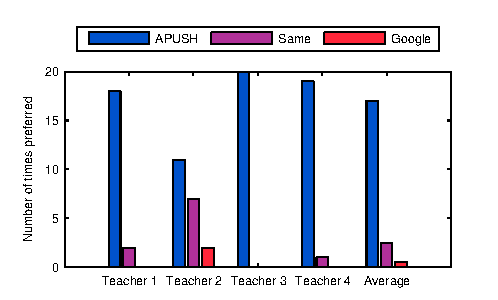
\includegraphics{teacher_eval}
\caption{Side-by-side comparison of the APUSH search engine and Google}
\label{fig-eval}
\end{figure}

We created a custom search engine using the good sites (available at
\url{http://guha.com/apushcse.html}) and evaluated it on a collection of 20
APUSH-related queries included in Appendix \ref{app-queries}.
We asked 4 history teachers to compare results from Google versus results
from the APUSH search engine in a blind side-by-side test. They were asked
to assign one of the following ratings to each side-by-side: side A/B is better,
side A/B are about the same. As can be seen in Figure \ref{fig-eval}, the
course-specific search engine is substantially preferred. 

\section{Methods for automation}

Instead of manually labeling thousands of sites, our goal to create a course-specific search engine from 
the course textbook with minimal manual supervision. We wish to develop algorithms that distinguish
between sites that produce off-topic results / sites that are inappropriate for 
academic usage and sites that may be used for academic work.  Rather than
attempting a binary classification of sites into ``good'' and ``bad'', we wish
to rank sites based on the likelihood of them returning good results for APUSH
searches. A search engine can then be configured to include just the top N sites
or better, or to prefer sites proportional to their likelihood of returning good
results in the APUSH context.

In order to automate the process of identifying these sites, we describe two
methods for using the authoritative content provided by the textbook. The main
intuition behind our algorithms is that by using the wealth of information
provided by the textbook, we can drastically improve upon generic search scoring
that is based solely on a two or three word query. 

\subsection{TF-IDF weighted text similarity}

We begin with an
approach that computes textual similarity between the textbook and a site via
TF-IDF weighted cosine distance. Classical 
information retrieval is based on the notion of similarity between two 
pieces of text---typically, the query and the web page.  Intuitively, by
preferring sites that are more similar to the APUSH textbook, the search engine
will be more likely to return better results for searches in the APUSH context.  

One of the most commonly used similarity measures is the cosine similarity
metric based on the vector space model of documents \cite{salton1975vector}. In
this model, each document is a vector in an $n$-dimensional space in which each
term in the corpus is a dimension. Using the popular TF-IDF weighting, the
magnitude of the document vector along the $i$th axis is given by by a product
of the term's frequency in the document (TF) and the inverse document frequency
(IDF) of the term---the log of the inverse fraction of documents containing the term in the
entire corpus. The cosine similarity between two documents in this space is
given by the angle between the document vectors.

In order to compute the similarity of a site to the APUSH textbook, we first
retrieve all pages from the site that are returned by Google for the queries
used to create the reference search engine. After stripping the pages of HTML
markup and javascript, we stem the words on each page (using the Porter stemmer 
\cite{porter1980algorithm}) and extract the terms from each along with their
frequency of occurrence. We sum the document vectors across the entire site and
compute the cosine similarity between the resulting site vector and that of
the APUSH textbook.

\subsection{Knowledge bases}

Next, we consider an approaching using
structured data from a knowledge base to identify APUSH-related categories,
entities and proper nouns. The realization that most queries and web documents
are about real word entities 
has led many of the major search engine providers to build various kinds of knowledge
bases to augment their search results (for example, see \cite{googlekg}). In the
academic sphere, there has also been significant work on the semantic
web \cite{berners2001semantic} and linked data \cite{bizer2008linked}, aiming to build a
large distributed network of information about entities and the relations
between them. In this section, we describe how knowledge bases can be
used to identify topics related to APUSH. The identification of these topics can
then be used improve ranking based on simple textual similarity.   

First, we observe that some types of entities lead to more off-topic results than
others. For example, places (e.g., Virginia, Maryland) are more likely to lead
to results that are not about history compared to US presidents since the former
will bring up real estate and local results. US presidents in turn are more
likely to bring up off-topic results compared to Confederate generals, since the
former are more likely to have institutions and places named after them. This
relative preference (Confederate generals better than US presidents better than
places) captures some of the APUSH context. 

Our goal is to automatically identify the types that are more likely to give
good results and give greater preference to the sites that contain these kinds
of entities. In order to do this, we must first construct mappings from the proper nouns that
we extract from the text to entities and from the entities to types of
entities. To construct such mappings in a fashion that is not specific to history, we need a
broad knowledge base about a large number of entities, along with information
about the type of each entity. Wikipedia contains such information and DBpedia
(available at \url{http://dbpedia.org/}) makes this information available as a
structured knowledge base. In particular, each ``thing'' in Wikipedia
corresponds to an entity in DBpedia and each ``category'' in Wikipedia
corresponds to a DBpedia type. We will use DBpedia as the primary source of
entities, types and for mapping proper nouns to entities and entities to types. 

Now we consider the task of mapping proper nouns extracted from text
to a set of candidate entities and types in DBpedia. In general, there are many
different proper nouns that refer to the same real world entity---for example,
President Lincoln, Abraham Lincoln, and Abe Lincoln all refer to the same 
person. Similarly, a given proper noun (e.g., Washington) could map to multiple
different entities. We found that the most robust way of mapping from proper
nouns to entities is to use search itself with the following method. For every
proper noun P, we issue the query [P site:wikipedia.org] which returns a set of
results with urls of the form ``http://\-en.wikipedia.org/wiki/<entity-id>''. We take
the top 3 entities for each query as the candidate entities for the corresponding
proper noun. Each entity may also have a number of categories associated with it---for  
example, the entity whose unique identifier is Abraham\_Lincoln has 29
different categories associated with it: American\_Presidents,
Illinois\_Lawyers, Assassinated\_HeadsOfState, etc. We use the RDF dumps from
DBpedia to construct the mapping from entities to categories.


Given these mappings from proper nouns to categories, we score each category
according to the likelihood of a query with proper nouns in that category
bringing up sites with on-topic results. The intuition behind the
scoring algorithm is as follows. A course, such as APUSH, is about certain
categories of entities and the relationships between them, for example
American\_Presidents. These categories should be assigned higher scores than
categories that appear only incidentally, such as Illinois\_Lawyers and
Noble\_titles. We would expect that a larger fraction of the entities in a
category that the course is about will occur in the textbook compared to
categories that appear incidentally. Thus we score a particular category with
the ratio
\begin{equation}
CategoryScore = \frac{\#Textbook}{\#DBpedia}
\end{equation}
where $\#Textbook$ and $\#DBpedia$ count the number of times entities in
the category occur in the textbook and DBpedia, respectively.

For example, the textbook contains references to 33 entities in the category
American\_Presidents, which, in DBpedia is associated with 44 entities, giving
this category a score of 0.75. On the other hand, even though the text contains
references to more Harvard\_University\_Alumni (34), a total of 6533 entities in
DBpedia are associated with this category, giving Harvard\_University\_Alumni a
much lower score than American\_Presidents. 

\begin{table}
\begin{center}
\begin{tabular}{|l|} \hline
19th-century presidents of the United States \\
United States Presidential Candidates \\
Oneida New York \\
Presidents of the United States \\
Whig Party \\
Presidency of James Monroe \\
Christian denominational families \\
\hline \end{tabular}
\caption{DBpedia categories for APUSH}
\label{tab-categories}
\end{center}
\end{table}

\begin{table}
\begin{center}
\begin{tabular}{|l|} \hline
Andrew Jackson \\
Martin Van Buren \\
Thomas Jefferson \\
James Monroe \\
Abraham Lincoln \\
James Buchanan \\
Zachary Taylor \\
William Henry Harrison \\
Russia \\
\hline\end{tabular}
\caption{DBpedia entities for APUSH}
\label{tab-entities}
\end{center}
\end{table}

Table \ref{tab-categories} gives top categories considered most relevant to
APUSH by this algorithm. As can be seen, of the hundreds of thousands of
categories in DBpedia (which includes categories for rock stars, planets, etc.), the
top scoring categories are indeed very apropos to US history.           


We then score each entity by summing the scores for the categories that it is
associated with. For example, the entity Abraham\_Lincoln gets a contribution
from each of the 29 categories that it is a part of. Table \ref{tab-entities}
gives the top-rated entities. 

\begin{table}
\begin{center}
\begin{tabular}{|l|} \hline
Whigs in Congress \\
President Harrison \\
President Monroe \\
James Monroe \\
President Johnson \\
Thomas Jefferson \\
President Adams \\
Second Bank \\
Andrew Jackson \\
President Van Buren \\
\hline\end{tabular}
\caption{Highest scoring proper terms for APUSH}
\label{tab-terms}
\end{center}
\end{table}



Next, we score each proper term by adding the scores of all the entities that it
could refer to. So, since ``Abraham Lincoln'' could refer to the president or the
movie with that name, each entity contributes a score. Table \ref{tab-terms}
gives the top-rated proper terms. Again, as can be seen, of the millions
of entries in DBpedia, the ones chosen are indeed very highly apropos to the
APUSH context.  


We then score each query by summing the scores of the proper terms in the query. Finally, we
score each of the sites based on the scores associated with the queries for
which they produced results. The score for the site is the average of the query
scores. This gives us a ranking of sites by the likelihood of them being a good
candidate for inclusion into the APUSH search engine. 

\subsection{Relevance feedback}

\begin{figure*}[t!]
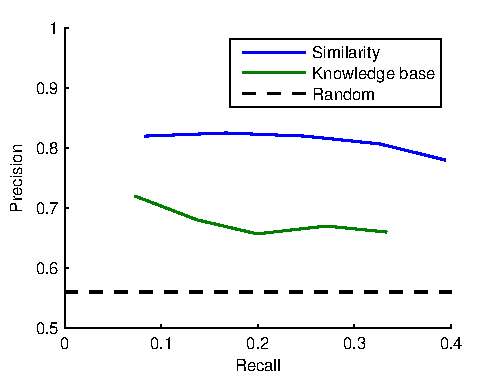
\includegraphics{expt}
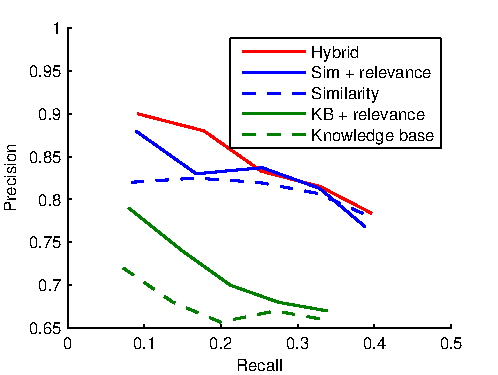
\includegraphics{expt_relevance}
\caption{Comparison of proposed algorithms on classification of APUSH
  sites (left); augmented with relevance feedback and hybrid scoring (right).
  Precision represents the percentage of good sites when looking at the
  top n sites and recall represents the percentage of good sites out of the
  total number of good sites that are in the top n } 
\label{fig-expt}
\end{figure*}

The previous two algorithms address the fundamental problem of off-topic search
results that we discuss in the introduction. As we demonstrate in the
experimental section, they both make significant progress toward automated
construction of the course-specific search engine for APUSH. However, they are
not well-suited to distinguish between good sites and sites that are on-topic
but either at the wrong academic level or inappropriate for academic purposes,
such as answers.yahoo.com or ConfederateAmericanPride.com. To address these
issues, we employ a classical method in information retrieval, relevance feedback.  

Using relevance feedback to improve the performance of systems is an established
technique \cite{salton1997improving}; as the search engine gets used, we can
interpret clicks from the user as feedback. For example, if users repeatedly
skip results from a certain site even when pages from that site are ranked
higher, preferring results from certain other sites, they are expressing a
judgement about the relevance of that site to the APUSH context. 

However, evaluating relevance feedback algorithms requires large amounts of
usage data, which is not available for a new search engine. Instead, we 
reuse the manually curated sites to evaluate the utility of relevance feedback
in our context. Of the sites that had been manually curated, we randomly
select 50 good and 50 bad sites. In practice, this list of good and bad
sites would be obtained from usage logs. 

In order to use relevance feedback to improve the text similarity algorithm, we
aggregate the text of the good sites and bad sites into two large composite documents. Then,
we score each site using TF-IDF weighted text similarity to generate a
$GoodScore$ and a $BadScore$ based on the site's similarity to each document. We
then form the $RelTextScore$ as  

\begin{equation}
RelTextScore = TextScore + GoodScore - BadScore
\end{equation}
where $GoodScore$ denotes the text similarity score between the site and the
document of good sites, $BadScore$ denotes the text similarity score between the
site and the document of bad sites, and $TextScore$ denotes the text similarity
score between the site and the APUSH textbook. $RelTextScore$ denotes the score
of a site based on it's textual similarity to the textbook and relevance
feedback. 

To augment the knowledge base approach, we compute a relevance feedback score
for each category as follows. We take the categories associated with each query 
and propagate them to the sites associated with the query to get
a set of categories associated with each site. The score associated with each
category is 
\begin{equation}
RelCategoryScore = CategoryScore + \#Good - \#Bad
\end{equation}
where $\#Good$ is the number of good sites associated with the category, $\#Bad$ is
the number of bad sites associated with the category, and $CategoryScore$ is the
category based score of each site (described and calculated in section 3.2)
. $RelCategoryScore$ represents the score of a category based on relevance
feedback.  
  
\section{Experimental results}

In this section, we evaluate the ability of our proposed methods to identify
high quality sites for a course-specific search engine. In practice, this
would typically be done using a side-by-side methodology to evaluate the
relative quality of search results similar to the procedure described in Section
2. However, given that the APUSH search engine constructed from a hand-labeled
corpus is strongly preferred to Google (as shown in Table \ref{fig-eval}), we
instead focus on the ability of our methods to recover this hand-labeled
corpus. For simplicity, we will evaluate our ranking of sites using a 
classification framework---of the 1757 APUSH-related sites, we consider what
fraction of the 989 good sites are ranked above the 768 bad ones.

In Figure \ref{fig-expt} (left) we see that both of our approaches significantly
outperform the baseline of $56\%$, which comes from picking sites
randomly. Although neither approaches provide perfect classification accuracy,
for the purposes of constructing a course-specific search engine, it is clear
that the course textbook provides a significant signal as to what is relevant
for the APUSH educational context.  Furthermore, the strongly positive
results of the side-by-side in Table \ref{fig-eval} suggest that even simplistic
methods of incorporating this signal into search ranking may lead to significant
gains in search quality.


In Figure \ref{fig-expt} (right), we examine the effect of incorporating
relevance feedback and hybrid scoring. We see that although relevance feedback
improves precision at various points on the recall curves---for example,
improving precision for the highest ranking sites from the knowledge base
approach---it does not have as large an impact as might be expected. We believe
the reasons for this are two-fold: 1) the simplistic nature of our use of the
feedback information and 2) a lack of real feedback data. Ideally, we would
improve on this result by using more sophisticated methods and a large amount of
real search logs from a running search engine. Finally, we also
investigate combining the textual similarity score with the knowledge base
score by simply adding the two scores. As can be seen, there
is a small improvement over just the similarity score and we believe that
improving this hybrid scoring is another direction for future work.

\section{Acknowledgments}

 We would like to thank Professor Lam and Dr. Hangal from Stanford for guiding
 our research and for feedback on several iterations of the paper. We would also
 like to thank Mr. Tuomy, Mr. Johnson, Ms. Richard and Mr. Weisman for taking
 the time to evaluate the search engine.

\bibliographystyle{abbrv}
\bibliography{apush_cse}

\appendix
\section{Side-by-side evaluation queries}
\label{app-queries}

In Table \ref{tab-queries} we list the queries used in our blind side-by-side
evaluation between the APUSH search engine and Google.


\begin{table}
\begin{center}
\begin{tabular}{|l|} \hline
Andrew Jackson \\
Battle of Saratoga \\
american strategies during world war 2 \\
andrew johnson reconstruction \\
battle of vicksburg \\
bay colony \\
british involvement civil war \\
carpetbaggers \\
causes of the civil war \\
great awakening \\
industrial revolution \\
king cotton \\
marne \\
mclellan \\
republicans reconstruction \\
sectionalism and slavery \\
tea party \\
uss chesapeake \\
war of 1812 \\
women's rights world war 2 \\
\hline\end{tabular}
\caption{Side-by-side evaluation queries}
\label{tab-queries}
\end{center}
\end{table}


\end{document}
